\section{Impulse Response Analysis}\label{sec:IRA}
    We calculated the orthogonal impulse response functions from Nelson-Siegel factors and they turned out to be insignificant (see \cref{fig:nsirf}). This implies that the 
    market segmentation hypothesis holds for the MOEX Russian government bond market.

    \begin{figure}[!h]
        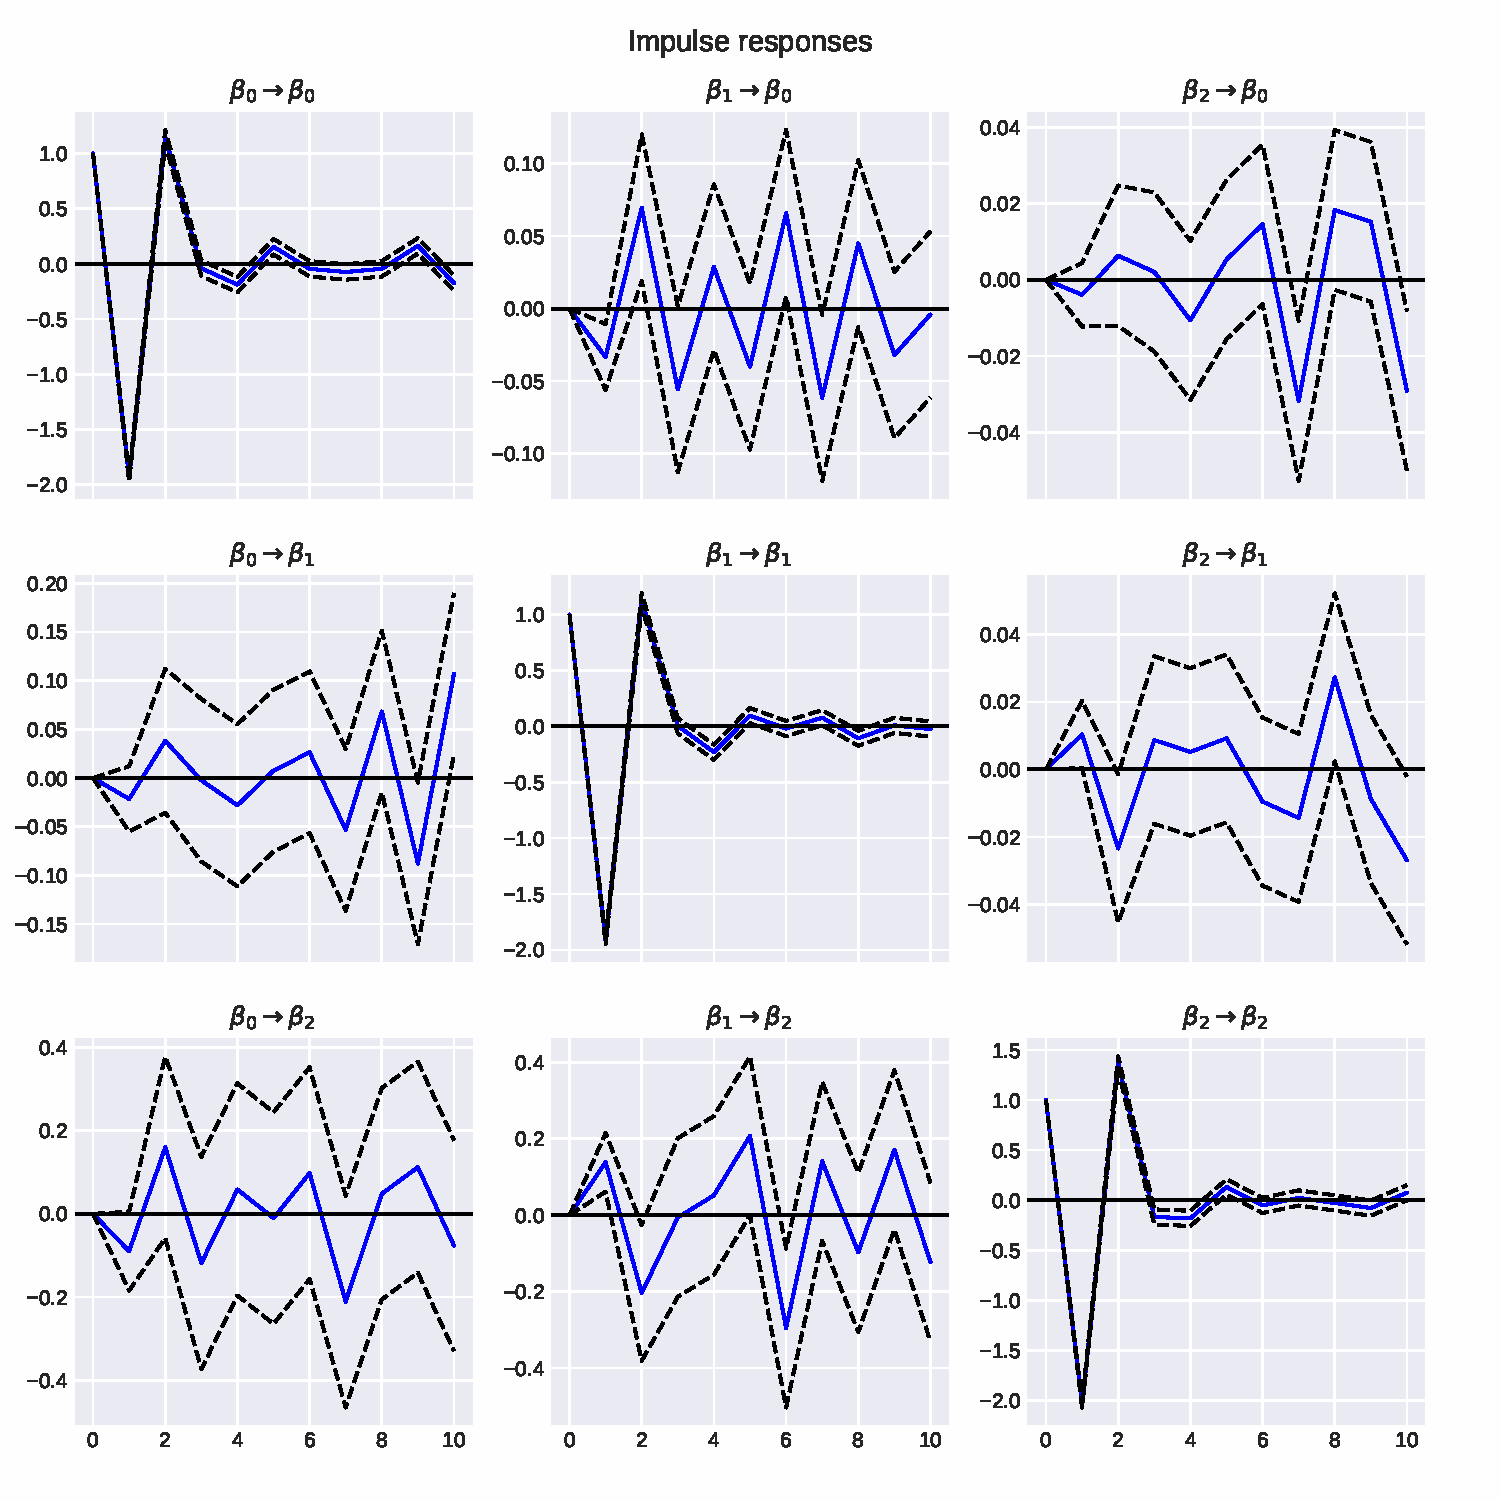
\includegraphics[width=\linewidth]{irfs.pdf}
        \caption{Nelson-Siegel impulse response functions.}
        \label{fig:nsirf}
    \end{figure}
